\documentclass[border=10pt,tikz]{standalone}
% Shared palette and styles for the Quota diagrams.
\usepackage{tikz}
\usepackage[T1]{fontenc}
\usepackage{helvet}
\renewcommand{\familydefault}{\sfdefault}
\usetikzlibrary{positioning,fit,backgrounds,arrows.meta,calc,shapes.geometric,shapes.symbols,decorations.pathreplacing,patterns}

\definecolor{qink}{HTML}{14110E}
\definecolor{qorange}{HTML}{E05A28}
\definecolor{qorangelt}{HTML}{FBE7DC}
\definecolor{qcream}{HTML}{FBF7F1}
\definecolor{qgrey}{HTML}{6B6560}
\definecolor{qline}{HTML}{C9C2B8}
\definecolor{qblue}{HTML}{1F5F8B}
\definecolor{qbluelt}{HTML}{DCE8F1}
\definecolor{qgreen}{HTML}{2F6B4F}
\definecolor{qgreenlt}{HTML}{DEEBE3}
\definecolor{qpaper}{HTML}{FFFFFF}

\tikzset{
  box/.style   = {rounded corners=2pt, draw=qline, line width=0.5pt, fill=qpaper,
                  align=center, inner sep=4pt, font=\scriptsize, text=qink},
  src/.style   = {box, minimum height=12mm, text width=25mm},
  proc/.style  = {box, minimum height=10mm, text width=30mm},
  gate/.style  = {box, draw=qorange, line width=1pt, fill=qorangelt},
  store/.style = {box, draw=qink, line width=0.8pt, fill=qcream},
  elas/.style  = {box, draw=qblue, line width=0.7pt, fill=qbluelt},
  human/.style = {box, draw=qgreen, line width=0.7pt, fill=qgreenlt},
  band/.style  = {font=\scriptsize\bfseries, text=qgrey, anchor=east, align=right},
  tag/.style   = {font=\tiny, text=qgrey, align=center, inner sep=1pt},
  ttl/.style   = {font=\scriptsize\bfseries, text=qink},
  flow/.style  = {-{Stealth[length=4pt,width=3pt]}, draw=qgrey, line width=0.7pt},
  flowo/.style = {-{Stealth[length=4pt,width=3pt]}, draw=qorange, line width=1pt},
  flowb/.style = {-{Stealth[length=4pt,width=3pt]}, draw=qblue, line width=0.9pt},
  flowg/.style = {-{Stealth[length=4pt,width=3pt]}, draw=qgreen, line width=0.9pt},
  dash/.style  = {draw=qline, line width=0.5pt, dash pattern=on 2pt off 2pt},
  grp/.style   = {rounded corners=3pt, draw=qline, line width=0.5pt, fill=qcream, inner sep=5pt},
}
\newcommand{\bb}[1]{\textbf{#1}}
\newcommand{\gy}[1]{{\color{qgrey}#1}}

\begin{document}
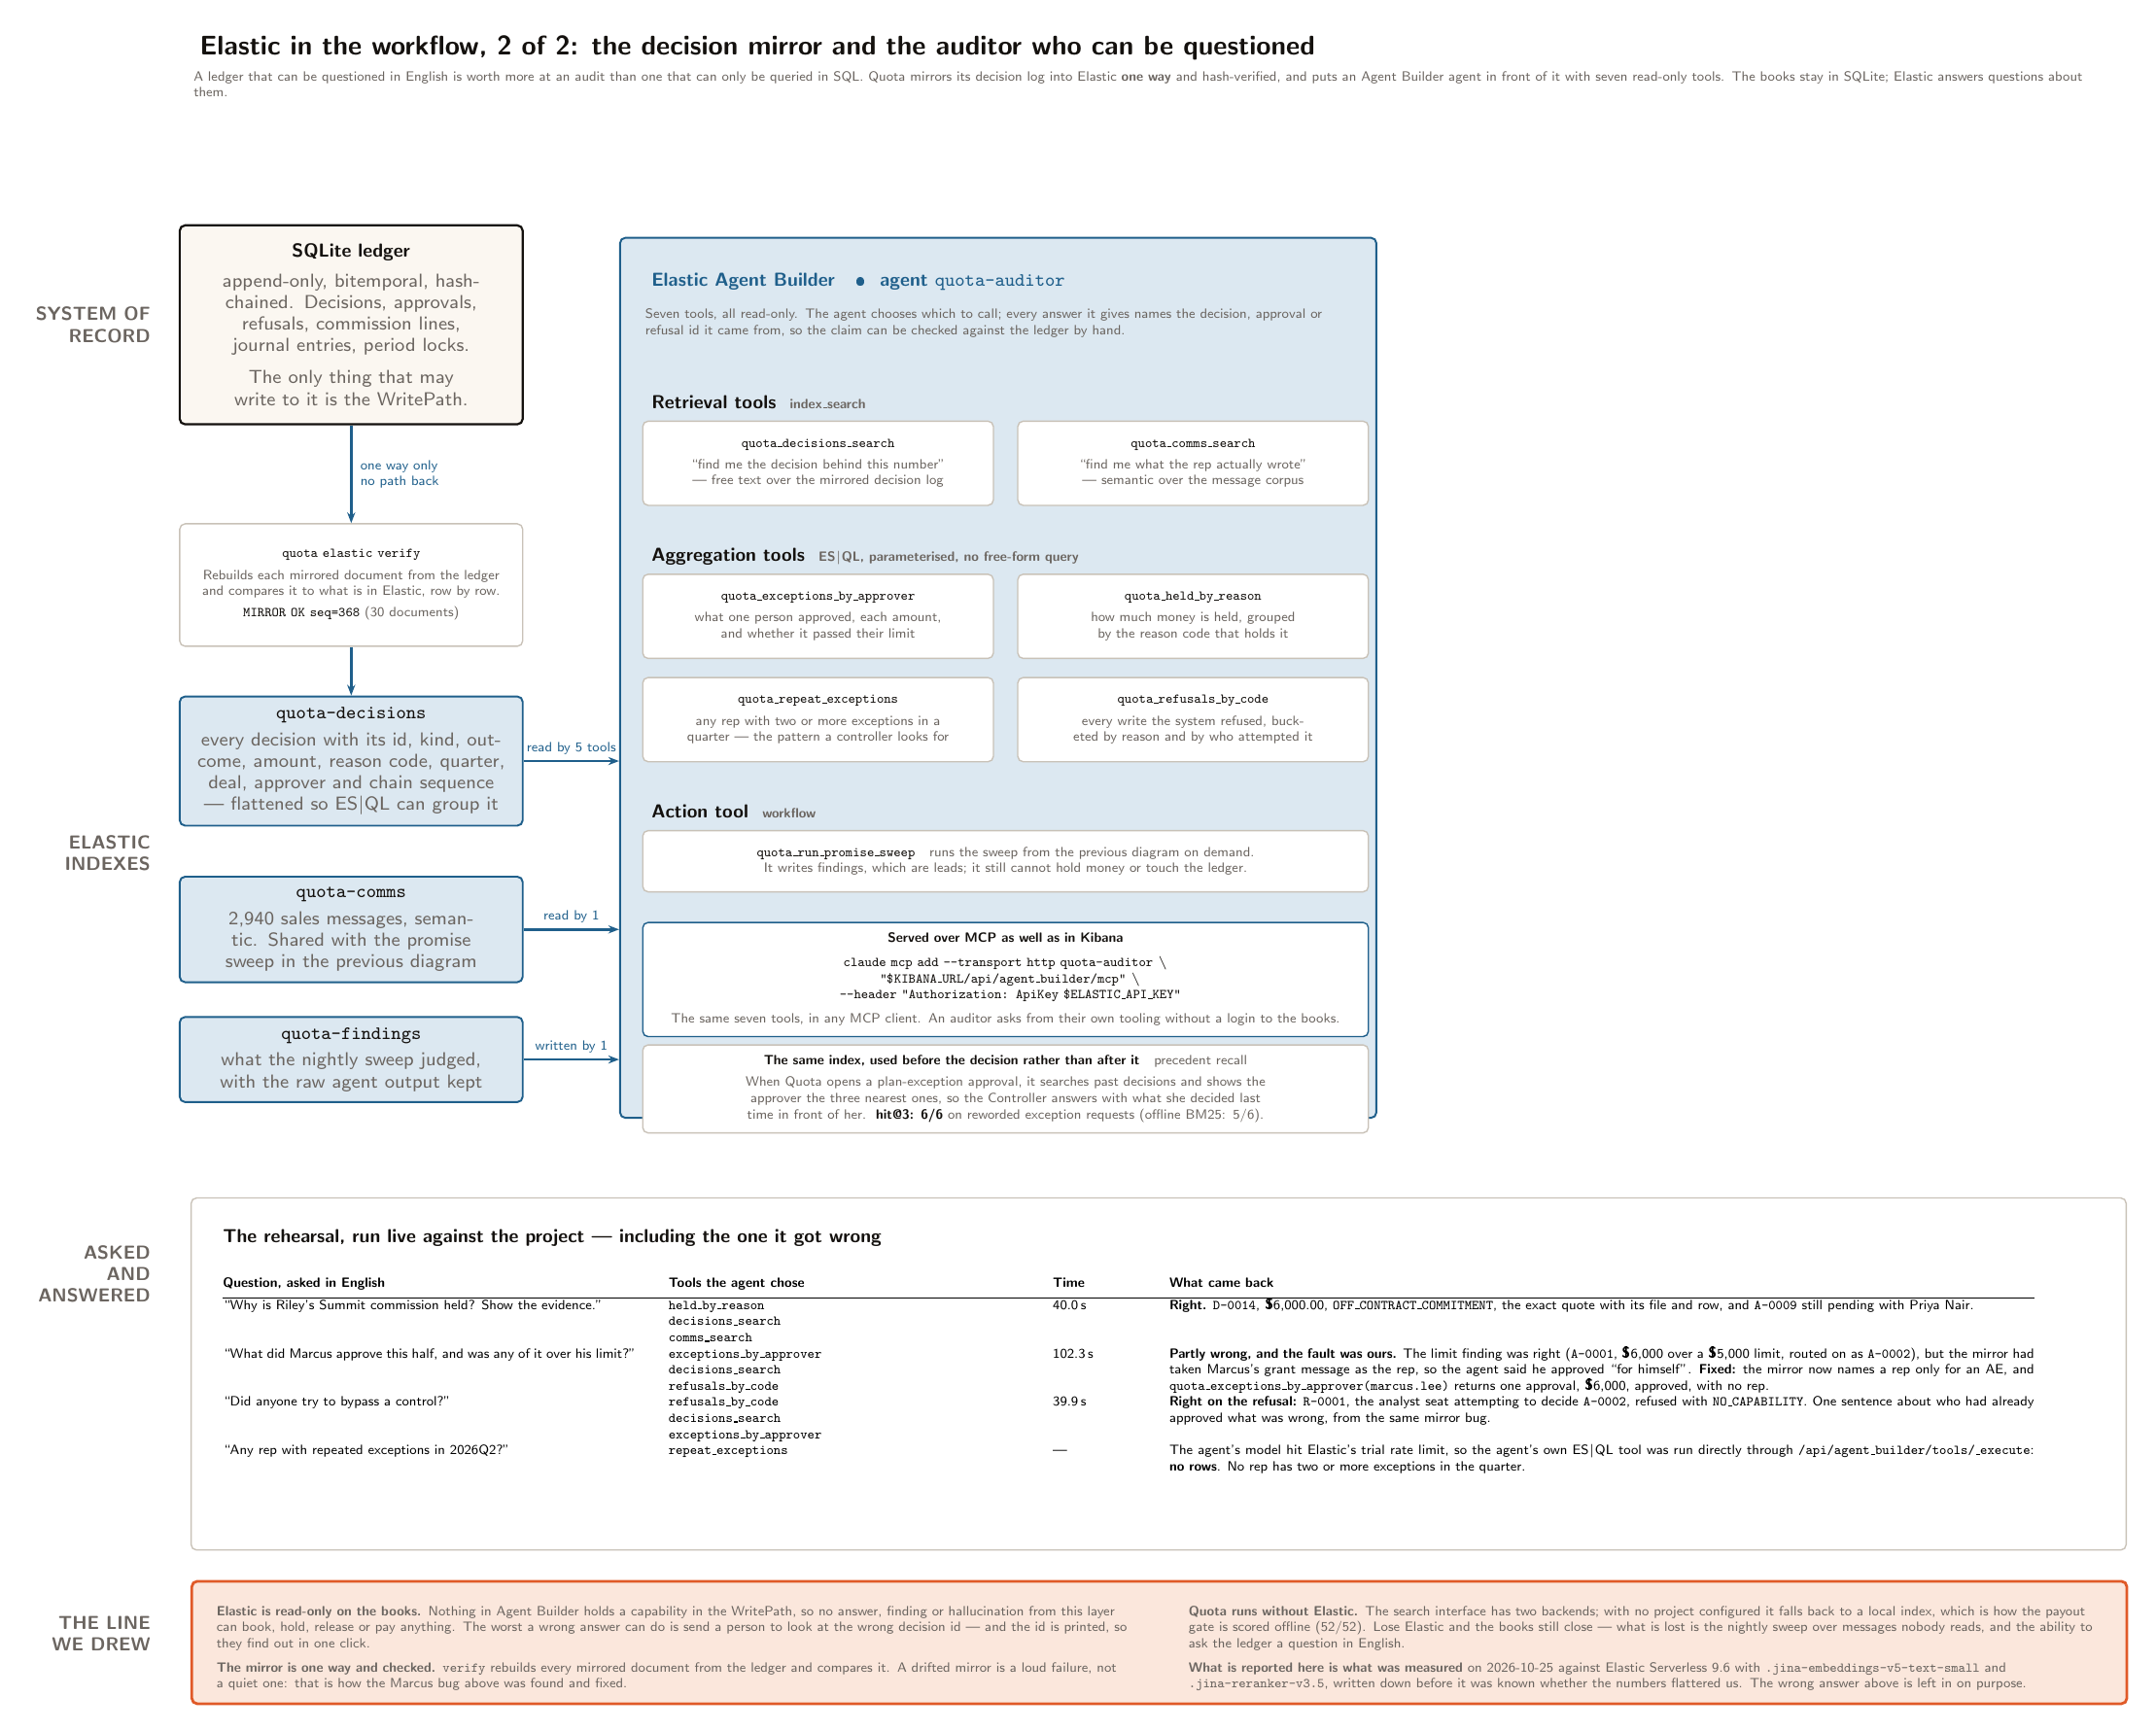
\begin{tikzpicture}[x=1cm,y=1cm]

\node[ttl, anchor=north west, font=\normalsize\bfseries] at (0,0.4) {Elastic in the workflow, 2 of 2: the decision mirror and the auditor who can be questioned};
\node[tag, anchor=north west, align=left, text width=250mm] at (0,-0.15)
  {{\color{qgrey}A ledger that can be questioned in English is worth more at an audit than one that can only be queried in SQL. Quota mirrors its decision log into Elastic \textbf{one way} and hash-verified, and puts an Agent Builder agent in front of it with seven read-only tools. The books stay in SQLite; Elastic answers questions about them.}};

%====================== LEDGER ======================
\node[band] at (-0.4,-3.5) {SYSTEM OF\\RECORD};
\node[store, text width=42mm, minimum height=26mm] at (2.1,-3.5) (led)
  {\bb{SQLite ledger}\\[3pt]{\color{qgrey}append-only, bitemporal, hash-chained. Decisions, approvals, refusals, commission lines, journal entries, period locks.}\\[4pt]
   {\color{qgrey}The only thing that may write to it is the WritePath.}};

\node[box, text width=42mm, minimum height=16mm, font=\tiny] at (2.1,-6.9) (mirror)
  {\bb{\texttt{quota elastic verify}}\\[2pt]{\color{qgrey}Rebuilds each mirrored document from the ledger and compares it to what is in Elastic, row by row.}\\[2pt]
   \bb{\texttt{MIRROR OK seq=368}} {\color{qgrey}(30 documents)}};
\draw[flowb] (led) -- node[tag,midway,right=2pt,font=\tiny,text=qblue,align=left]{one way only\\no path back} (mirror);

%====================== INDEXES ======================
\node[band] at (-0.4,-10.4) {ELASTIC\\INDEXES};
\node[elas, text width=42mm, minimum height=15mm] at (2.1,-9.2) (dec)
  {\bb{\texttt{quota-decisions}}\\[2pt]{\color{qgrey}every decision with its id, kind, outcome, amount, reason code, quarter, deal, approver and chain sequence \textemdash{} flattened so ES\textbar{}QL can group it}};
\node[elas, text width=42mm, minimum height=11mm] at (2.1,-11.4) (comms)
  {\bb{\texttt{quota-comms}}\\[2pt]{\color{qgrey}2{,}940 sales messages, semantic. Shared with the promise sweep in the previous diagram}};
\node[elas, text width=42mm, minimum height=9mm] at (2.1,-13.1) (find)
  {\bb{\texttt{quota-findings}}\\[2pt]{\color{qgrey}what the nightly sweep judged, with the raw agent output kept}};
\draw[flowb] (mirror) -- (dec);

%====================== AGENT BUILDER ======================
\node[elas, text width=96mm, minimum height=115mm, anchor=north west] at (5.6,-2.35) (ab) {};
\node[ttl, anchor=north west, text=qblue] at (5.9,-2.7) {Elastic Agent Builder \ \ \textbullet\ \ agent \texttt{quota-auditor}};
\node[tag, anchor=north west, align=left, text width=92mm] at (5.9,-3.25)
  {{\color{qgrey}Seven tools, all read-only. The agent chooses which to call; every answer it gives names the decision, approval or refusal id it came from, so the claim can be checked against the ledger by hand.}};

\node[ttl, anchor=north west, font=\scriptsize\bfseries] at (5.9,-4.3) {Retrieval tools \ {\color{qgrey}\tiny index\_search}};
\node[box, text width=43mm, minimum height=11mm, font=\tiny, anchor=north west] at (5.9,-4.75) (t1)
  {\bb{\texttt{quota\_decisions\_search}}\\[2pt]{\color{qgrey}``find me the decision behind this number'' \textemdash{} free text over the mirrored decision log}};
\node[box, text width=43mm, minimum height=11mm, font=\tiny, anchor=north west] at (10.8,-4.75) (t2)
  {\bb{\texttt{quota\_comms\_search}}\\[2pt]{\color{qgrey}``find me what the rep actually wrote'' \textemdash{} semantic over the message corpus}};

\node[ttl, anchor=north west, font=\scriptsize\bfseries] at (5.9,-6.3) {Aggregation tools \ {\color{qgrey}\tiny ES\textbar{}QL, parameterised, no free-form query}};
\node[box, text width=43mm, minimum height=11mm, font=\tiny, anchor=north west] at (5.9,-6.75) (t3)
  {\bb{\texttt{quota\_exceptions\_by\_approver}}\\[2pt]{\color{qgrey}what one person approved, each amount, and whether it passed their limit}};
\node[box, text width=43mm, minimum height=11mm, font=\tiny, anchor=north west] at (10.8,-6.75) (t4)
  {\bb{\texttt{quota\_held\_by\_reason}}\\[2pt]{\color{qgrey}how much money is held, grouped by the reason code that holds it}};
\node[box, text width=43mm, minimum height=11mm, font=\tiny, anchor=north west] at (5.9,-8.1) (t5)
  {\bb{\texttt{quota\_repeat\_exceptions}}\\[2pt]{\color{qgrey}any rep with two or more exceptions in a quarter \textemdash{} the pattern a controller looks for}};
\node[box, text width=43mm, minimum height=11mm, font=\tiny, anchor=north west] at (10.8,-8.1) (t6)
  {\bb{\texttt{quota\_refusals\_by\_code}}\\[2pt]{\color{qgrey}every write the system refused, bucketed by reason and by who attempted it}};

\node[ttl, anchor=north west, font=\scriptsize\bfseries] at (5.9,-9.65) {Action tool \ {\color{qgrey}\tiny workflow}};
\node[box, text width=92mm, minimum height=8mm, font=\tiny, anchor=north west] at (5.9,-10.1) (t7)
  {\bb{\texttt{quota\_run\_promise\_sweep}} \ \ {\color{qgrey}runs the sweep from the previous diagram on demand. It writes findings, which are leads; it still cannot hold money or touch the ledger.}};

\node[box, draw=qblue, fill=qpaper, text width=92mm, minimum height=13mm, font=\tiny, anchor=north west] at (5.9,-11.3) (mcp)
  {\bb{Served over MCP as well as in Kibana}\\[3pt]
   \texttt{claude mcp add --transport http quota-auditor \textbackslash}\\
   \texttt{\ \ "\$KIBANA\_URL/api/agent\_builder/mcp" \textbackslash}\\
   \texttt{\ \ --header "Authorization: ApiKey \$ELASTIC\_API\_KEY"}\\[3pt]
   {\color{qgrey}The same seven tools, in any MCP client. An auditor asks from their own tooling without a login to the books.}};

\node[box, text width=92mm, minimum height=10mm, font=\tiny, anchor=north west] at (5.9,-12.9) (prec)
  {\bb{The same index, used before the decision rather than after it} \ \ {\color{qgrey}precedent recall}\\[2pt]
   {\color{qgrey}When Quota opens a plan-exception approval, it searches past decisions and shows the approver the three nearest ones, so the Controller answers with what she decided last time in front of her.}\ \ \bb{hit@3: 6/6} {\color{qgrey}on reworded exception requests (offline BM25: 5/6).}};

\draw[flowb] (dec.east)   -- node[tag,midway,above=1pt,font=\tiny,text=qblue]{read by 5 tools} (ab.west|-dec);
\draw[flowb] (comms.east) -- node[tag,midway,above=1pt,font=\tiny,text=qblue]{read by 1} (ab.west|-comms);
\draw[flowb] (find.east)  -- node[tag,midway,above=1pt,font=\tiny,text=qblue]{written by 1} (ab.west|-find);

%====================== THE REHEARSAL ======================
\node[band] at (-0.4,-15.9) {ASKED\\AND\\ANSWERED};
\node[box, text width=250mm, minimum height=46mm, anchor=north west] at (0,-14.9) (reh) {};
\node[ttl, anchor=north west] at (0.3,-15.2) {The rehearsal, run live against the project \textemdash{} including the one it got wrong};
\node[anchor=north west, font=\tiny] at (0.3,-15.8) {%
\begin{tabular}{@{}p{54mm}p{46mm}p{11mm}p{113mm}@{}}
\textbf{Question, asked in English} & \textbf{Tools the agent chose} & \textbf{Time} & \textbf{What came back}\\[2pt]
\hline\\[-6pt]
``Why is Riley's Summit commission held? Show the evidence.''
  & \texttt{held\_by\_reason}\newline \texttt{decisions\_search}\newline \texttt{comms\_search} & 40.0\,s
  & \textbf{Right.} \texttt{D-0014}, \$6{,}000.00, \texttt{OFF\_CONTRACT\_COMMITMENT}, the exact quote with its file and row, and \texttt{A-0009} still pending with Priya Nair.\\[4pt]
``What did Marcus approve this half, and was any of it over his limit?''
  & \texttt{exceptions\_by\_approver}\newline \texttt{decisions\_search}\newline \texttt{refusals\_by\_code} & 102.3\,s
  & \textbf{Partly wrong, and the fault was ours.} The limit finding was right (\texttt{A-0001}, \$6{,}000 over a \$5{,}000 limit, routed on as \texttt{A-0002}), but the mirror had taken Marcus's grant message as the rep, so the agent said he approved ``for himself''. \textbf{Fixed:} the mirror now names a rep only for an AE, and \texttt{quota\_exceptions\_by\_approver(marcus.lee)} returns one approval, \$6{,}000, approved, with no rep.\\[4pt]
``Did anyone try to bypass a control?''
  & \texttt{refusals\_by\_code}\newline \texttt{decisions\_search}\newline \texttt{exceptions\_by\_approver} & 39.9\,s
  & \textbf{Right on the refusal:} \texttt{R-0001}, the analyst seat attempting to decide \texttt{A-0002}, refused with \texttt{NO\_CAPABILITY}. One sentence about who had already approved what was wrong, from the same mirror bug.\\[4pt]
``Any rep with repeated exceptions in 2026Q2?''
  & \texttt{repeat\_exceptions} & \textemdash
  & The agent's model hit Elastic's trial rate limit, so the agent's own ES\textbar{}QL tool was run directly through \texttt{/api/agent\_builder/tools/\_execute}: \textbf{no rows}. No rep has two or more exceptions in the quarter.\\
\end{tabular}};

%====================== BOUNDARY ======================
\node[band] at (-0.4,-20.6) {THE LINE\\WE DREW};
\node[box, draw=qorange, line width=1pt, fill=qorangelt, text width=250mm, minimum height=16mm, anchor=north west] at (0,-19.9) (bnd) {};
\node[tag, anchor=north west, align=left, text width=119mm] at (0.3,-20.2)
  {\bb{Elastic is read-only on the books.} {\color{qgrey}Nothing in Agent Builder holds a capability in the WritePath, so no answer, finding or hallucination from this layer can book, hold, release or pay anything. The worst a wrong answer can do is send a person to look at the wrong decision id \textemdash{} and the id is printed, so they find out in one click.}\\[3pt]
  \bb{The mirror is one way and checked.} {\color{qgrey}\texttt{verify} rebuilds every mirrored document from the ledger and compares it. A drifted mirror is a loud failure, not a quiet one: that is how the Marcus bug above was found and fixed.}};
\node[tag, anchor=north west, align=left, text width=119mm] at (13.0,-20.2)
  {\bb{Quota runs without Elastic.} {\color{qgrey}The search interface has two backends; with no project configured it falls back to a local index, which is how the payout gate is scored offline (52/52). Lose Elastic and the books still close \textemdash{} what is lost is the nightly sweep over messages nobody reads, and the ability to ask the ledger a question in English.}\\[3pt]
  \bb{What is reported here is what was measured} {\color{qgrey}on 2026-10-25 against Elastic Serverless 9.6 with \texttt{.jina-embeddings-v5-text-small} and \texttt{.jina-reranker-v3.5}, written down before it was known whether the numbers flattered us. The wrong answer above is left in on purpose.}};

\end{tikzpicture}
\end{document}
